\documentclass{ubicomp2013}
\usepackage{times}
\usepackage{url}
\usepackage{graphics}
\usepackage{color}
\usepackage[pdftex]{hyperref}
\hypersetup{%
pdftitle={An Ontology Based Sensor Selection Engine
}, pdfauthor={Prajit Kumar Das, Primal Pappachan}, pdfkeywords={ontology, sensor, selection}, bookmarksnumbered, pdfstartview={FitH}, colorlinks,
citecolor=black, filecolor=black, linkcolor=black, urlcolor=black,
breaklinks=true, }
\newcommand{\comment}[1]{}
\definecolor{Orange}{rgb}{1,0.5,0}
\newcommand{\todo}[1]{\textsf{\textbf{\textcolor{Orange}{[[#1]]}}}}

%\pagenumbering{arabic}  % Arabic page numbers for submission.  Remove this line to eliminate page numbers for the camera ready copy

\begin{document}
% to make various LaTeX processors do the right thing with page size
\special{projectsize=8.5in,11in}
\setlength{\projectheight}{11in}
\setlength{\projectwidth}{8.5in}
\setlength{\pdfpageheight}{\projectheight}
\setlength{\pdfpagewidth}{\projectwidth}

% use this command to override the default ACM copyright statement
% (e.g. for preprints). Remove for camera ready copy.
%\toappear{Submitted for review to UbiComp 2013.}

\title{An Ontology Based Sensor Selection Engine}
\numberofauthors{2}
\author{
  \alignauthor Prajit Kumar Das\\
    \affaddr{University of Maryland, Baltimore County}\\
    \email{prajit1@umbc.edu}  \\
   \alignauthor Primal Pappachan\\
    \affaddr{University of Maryland, Baltimore County}\\
    \email{primal1@umbc.edu} }
\maketitle

\begin{abstract}

In this project we describe the base ontology that would define sensors as a generic concept while at the same time, being applicable to sensors on a modern mobile smartphone. We used an ontology, in this project, to define the hierarchical concept of sensors on a smartphone. We are using the ontology to introduce the generic properties of sensors that allows us to select the best among the ones available to us. The criterion for the selection being the accuracy of the sensor and energy efficiency rating or energy cost of the sensor. The project is part of our research work, where we are creating a context-aware, energy efficient middleware on an Android smartphone. The primary motivation of this work comes from the domain of context-aware privacy management on mobile devices. Fine-grained, policy based, privacy management can be done in a better manner if the user's context is known at every time instant. However, in doing so we would drain out the battery of the mobile. Thus we propose a technique for managing the energy costs too. 

\end{abstract}

\keywords{Semantic Web, Ontology, Sensor Selection, Context-aware, Energy Efficient}

\section{Introduction}

Contemporary enterprise work environments are witnessing a significant rise in accommodation or adoption of the Bring-Your-Own-Device (BYOD) model. Concerns over corporate data protection has led to security firms actively researching the challenges and opportunities of using such a model. Ionic Security, an Atlanta based startup recently raised \$9.4 million to develop its technology for enabling employees to access data on their own devices \cite{harris2013byod}. The focus of privacy or security firms has remained on securing the data in case of loss of the device \cite{goldberg2013byod} or IT implementation and economic challenges \cite{guptill2013byod}. One approach for providing privacy to corporate data is the container based approach. Samsung and Blackberry, through their SAFE (SAmsung For Enterprises) \cite{honig2013knox} and Balance \cite{halliwell2013balance} systems 
provided separate containers for corporate data. Container based approaches provide security to corporate data but with larger overheads of security enhanced operating systems and separate application groups.

However, container based systems ignore user context data flow and modern smartphones are capable of much more than just storing corporate data i.e. they can gather tremendous amounts of information about the user and her context. User data and context leakage thus, becomes an enormous issue with potentially disastrous results. Naturally, we recognized the move to BYOD model as a major challenge, making privacy management on smartphones an important goal. Advances made in context modeling, location tracking and collaborative localization has resulted in emergence of a class of smartphone apps that can access and share embedded sensor and context data. Current security and privacy mechanisms on Android and other mobile operating systems are not well equipped to handle dynamic data flow between the framework and the applications.

In our previous work, we have shown application and user context-dependent information sharing policies that dynamically control data flow among applications at a fine-grained level\footnote{Application and App are both used to refer to the same concept, of an Android App in this project}. We use semantically rich policies to dynamically monitor and control the data flow between the sensors and the apps on a smartphone \cite{ghosh2012ms}. This second approach to privacy management is finer grained and more robust and carries less overhead than container based systems described above.

The other challenge apart from privacy management comes from the separate but equally vital problem of limited battery capacity, on smartphones. Users' expectations from their smartphones are increasing every day and thus the need for them to do more computation is also increasing. However, the ability of batteries to power these devices are not increasing as fast as the processing capabilities \cite{boxall2012battery}. Therefore, there is a necessity to preserve the battery as much as possible, thus extending the battery life.

While policy based privacy management has its advantages, it does require the latest context to be available at all times. Therefore necessitating context update at a high frequency. This unfortunately creates a serious hindrance due to the limited battery capacity on smartphones. We created an app that would update the context (location using GPS) with a high frequency and found out that the battery can drain out as fast as five hours, given certain conditions are true. Energy efficient privacy management therefore becomes, an important goal. In our ongoing work we have presented a three-fold solution towards achieving this ultimate goal \cite{das2012energy}. In this project we focus on the creation of the ontology for carrying out these tasks.

\begin{figure*}[tbh]
\centering
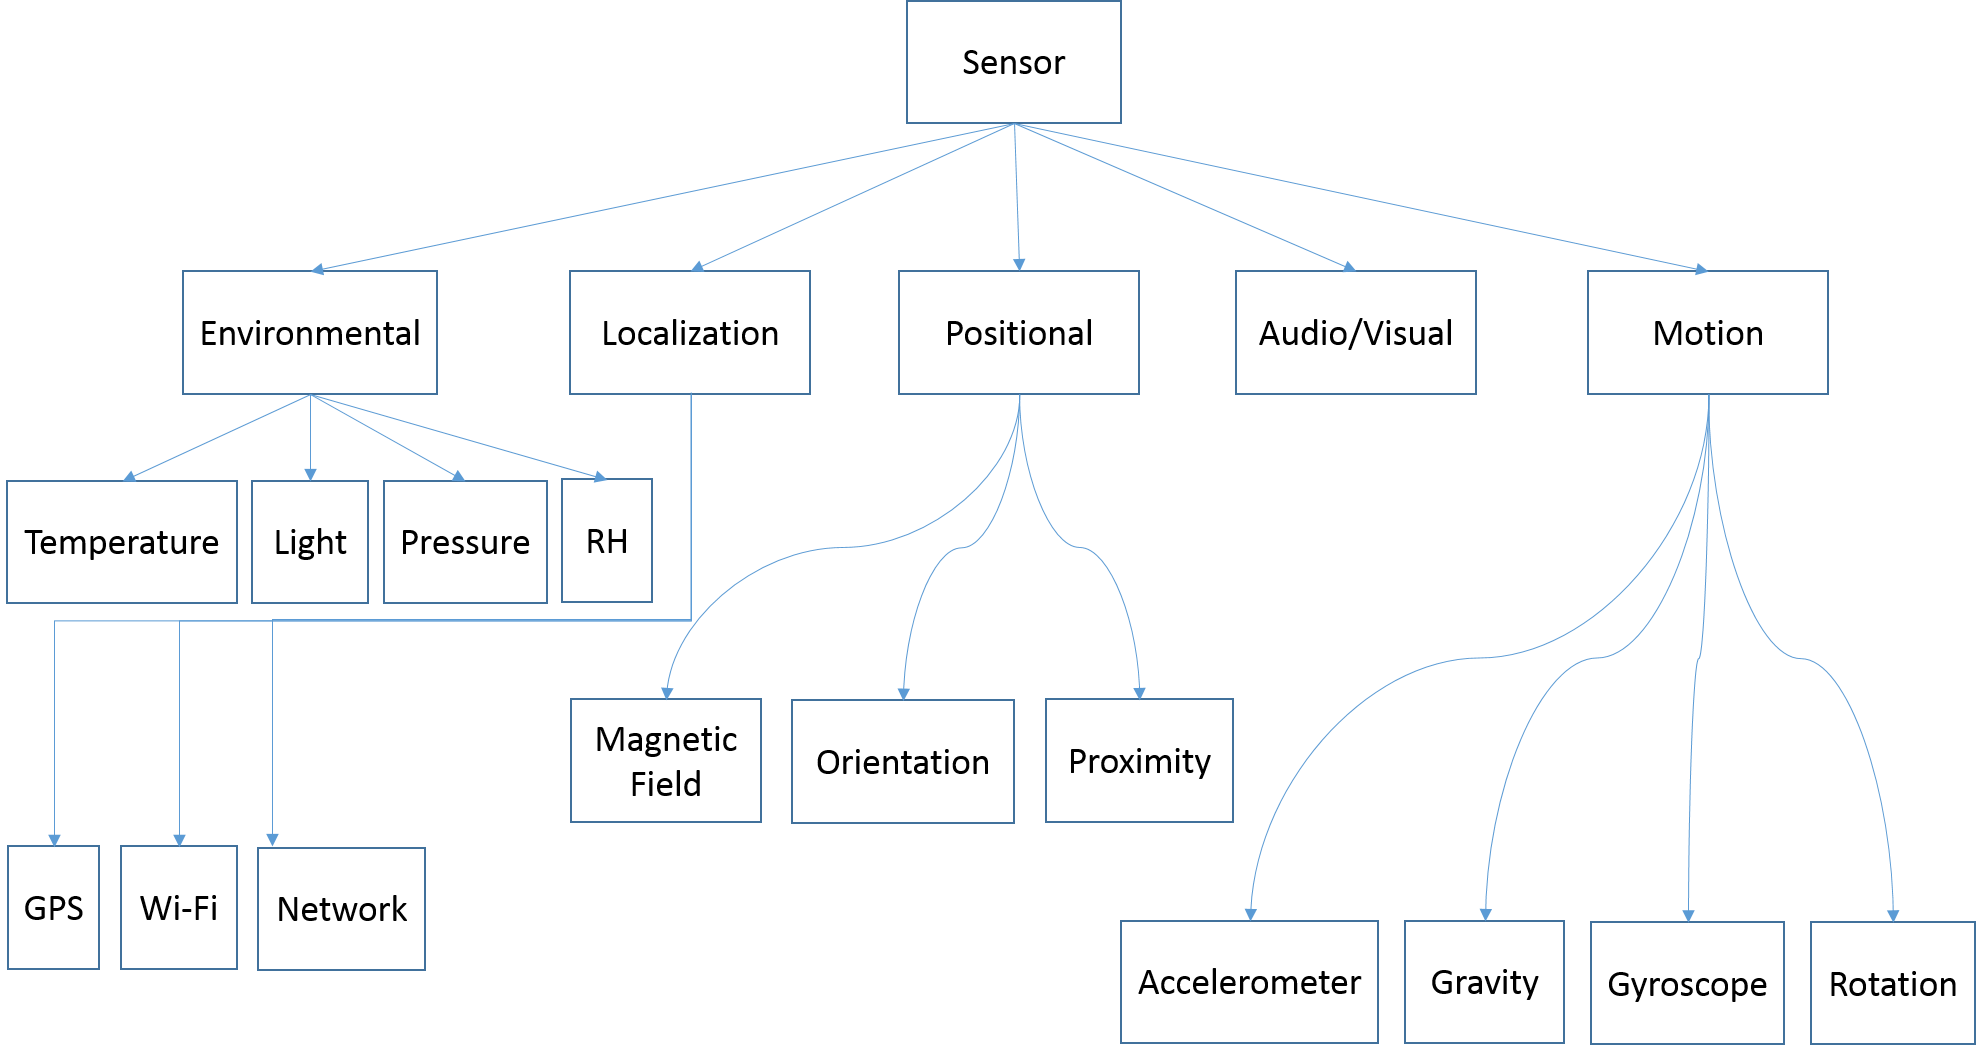
\includegraphics[width=0.9\textwidth]{Sensor_Class_Hierarchy.png}
\caption{Shows the sensor class hierarchy that we are trying to define using the ontology}
\label{fig:hierarchy}
\end{figure*}

In this project we focus on the sub-solution of sensor selection to achieve energy efficiency. We show the architecture diagram of the COntext MANager miDDleware (COMANDD) for achieving the sub-goal. We extend a mobile ontology i.e. PlatMob \cite{ghosh2012privacy,ghosh2012ms} from our previous work to include the concept of a sensor on a device and represent a sensor's capability (the type of data it senses), accuracy level (precision of the sensor) and energy cost (the energy cost of the sensor) as seen in Figure \ref{fig:hierarchy}.
  
In our research we came up with a three-fold solution to this problem. We are focusing on a single part of this three-fold solution in this project. We extend the concepts of user activity and location notion defined in the Platys project to include the idea of a temporal activity expiration and dirty context information. Our approach to reducing energy costs is by reasoning about what context information is known, what additional information is needed, how accurate it must be and how to efficiently acquire it. We model the sensors and their data properties, accuracy levels and energy costs in a knowledge base supported by an ontology. We describe a method to manage privacy on smartphones in an energy efficient manner by selecting the best choice sensor for maintaining the user's context information. Sensor selection is done by COntext MANager miDDleware (COMANDD), which maintains a context model and answers queries about it. Context requests are served by capability matching, accuracy level matching and selection of lowest energy cost sensor for reporting context data. A context change detection function is used to decide when the context should be updated.

The rest of the project report is organized as follows. Section 2 explains the three-fold energy efficiency solution design. Section 3 dives into the sub-solution of sensor selection and describes the ontology that allows us to select a sensor using an example rule. Section 4 describes the methodology used for the creation of the energy model and relative accuracy values of location sensors. Section 5 summarizes the related work from the literature. Section 6 summarizes the ongoing work and concludes the project. 

\section{Previous Work}
{\em Privacy management:} Our approach for privacy management differs from those in the literature \cite{conti2011crepe, sadeh2003mycampus, enck2010taintdroid} on context based privacy and security.  Using semantically rich policies and the user and user application context we undertake a reasoning method to decide the choice of either releasing or obfuscating the sensor/context data being shared with the application \cite{ghosh2012ms, ghosh2012privacy, palani2012infoflow}. We obtain rich context mapping between a location and its surroundings, the presence of people and devices, inferred activities and the roles people fill in them. All the facts are inferred by a model created by using a machine learning system trained on user data \cite{zavala2011mobile}. The context realized as a dynamic knowledge-base of RDF triples is grounded in an ontology expressed in the semantic web language OWL. All policies are encoded in form of SWRL \cite{horrocks2004swrl} rules and use conjunctions of facts in the context knowledge-base in their conditions. The rules control the sensor data flow from the Android framework to the requesting app. When policies necessitate protection of certain data flow form sensors to an app the data is obfuscated. Our ontology represents the concept of application provenance that is used in policies. The resulting system provides fine-grained, context-dependent control to sensitive user data \cite{ghosh2012ms}. 

{\em Energy efficiency:} Current work in the literature on the energy
consumption study focuses on exact battery utilization of specific
applications and also refers to tail energy issues
\cite{pathak2011finegrainedenergy}, but has not dealt with creating an
energy efficient context inference system that can be used for
security.  In ongoing work we have carried out studies on Android
smartphones to find out energy consumption pattern of individual
sensors and their accuracy values. \cite{das2012energy}. We group
sensors according to the type of data they sense. Android's developer
documentation has a basic classification of the sensor categories
\cite{android2013sesnors}, i.e. Motion, Position and Environment. The
context data we are trying to infer or gather or pass includes a
fourth category of sensors called Location. We utilize the
localization capable components as sensors in this case.

Acquisitional Context Engine (ACE) is a work done in energy efficient context inference. This work includes the notion of {\em Inference Caching} and {\em Context Correlation Mining}. In our current work we have adopted a unique approach of defining a function that would specify that the context is outdated and needs to be updated. Given an initial location and activity context, we use a function with inputs of activity length, current time and a low cost motion sensor like accelerometer to determine whether there was any change in context or not. Thus we avoid updating context altogether by using a low energy costing sensor and avoid the need to maintain a caching mechanism.

\section{Ongoing Work}
In this project we have provided a design of an energy efficient privacy management solution. We are in process of implementing the middleware for which we have provided the design here. Evaluation of the system poses to be a challenge. We plan to implement two separate systems with and without the context manager middleware and compare and contrast the results to evaluate our system for various privacy manager use cases.

The research work done here is based on the data that can be successfully obtained using Android framework provided data. The best precision of data available through the framework is a one percent change in the battery level. Although the expected battery drain is linear. It may not be exactly linear. We are working on other phones and carrying out research by varying the parameters that affect accuracy and efficiency. We eventually intend to collect enough data to run a learning algorithm and generate a model file. When this model would be put on a phone it will be able to predict the energy consumption patterns of the phones components and adjust the model if necessary.

In course of our research, we observed that frequent update to location context had a significant impact on the battery. GPS position fix although takes substantial time initially \cite{liu2012gps} but once obtained, provides high accuracy in location information. Wi-Fi, on the other hand, had relatively lower precision but got initial position fix faster at known Wi-Fi access point locations. We do take advantage of this trade-off of location precision versus energy measurements to optimize our energy efficiency algorithm. But we have not considered the time to obtain this fix with respect to energy consumption. We would like to study this aspect in the future. We have created the policy-based security mechanism in the Android framework \cite{ghosh2012ms, ghosh2012privacy} and have designed and partially implemented the energy efficient privacy framework. Evaluating this system, however remains to be done.

\section{Platys Ontology Description}

In order to make a system on a mobile, energy efficient and making selections of sensors to be based upon energy cost of individual sensors, it is first and foremost necessary to explore the energy consumption of individual components on a smartphone. Towards that goal we created an Android app capable of collecting data of current battery levels. The app records any change in battery levels along with the timestamps and stores the information on an external storage on the phone. We created a baseline for the bare bone Android system in airplane mode. This ensured that there was no network communication. We also ensured that no other apps were running on the system. Using Android programming constructs we ensured that the system was running only the operating system on its own and nothing else. We drained the battery out in this condition. Our technique thus provided us with battery consumption pattern which formed the baseline for our energy model.

Creation of the energy model that was carried out included the task of selecting a component that we wanted to model. Selection was done for all possible sensors in each individual sensor group (mentioned in previous section). Once a component was selected we yet again used an Android app to run that component, refreshing the data obtained over small time intervals and storing the battery level changes, timestamps and the sensor data obtained. At present we have created models for location detection sensors. Figure \ref{fig:battery} shows the comparative battery drainage time for Wi-Fi, Network, GPS and the baseline system.
  
\begin{figure*}[tbh]
\centering
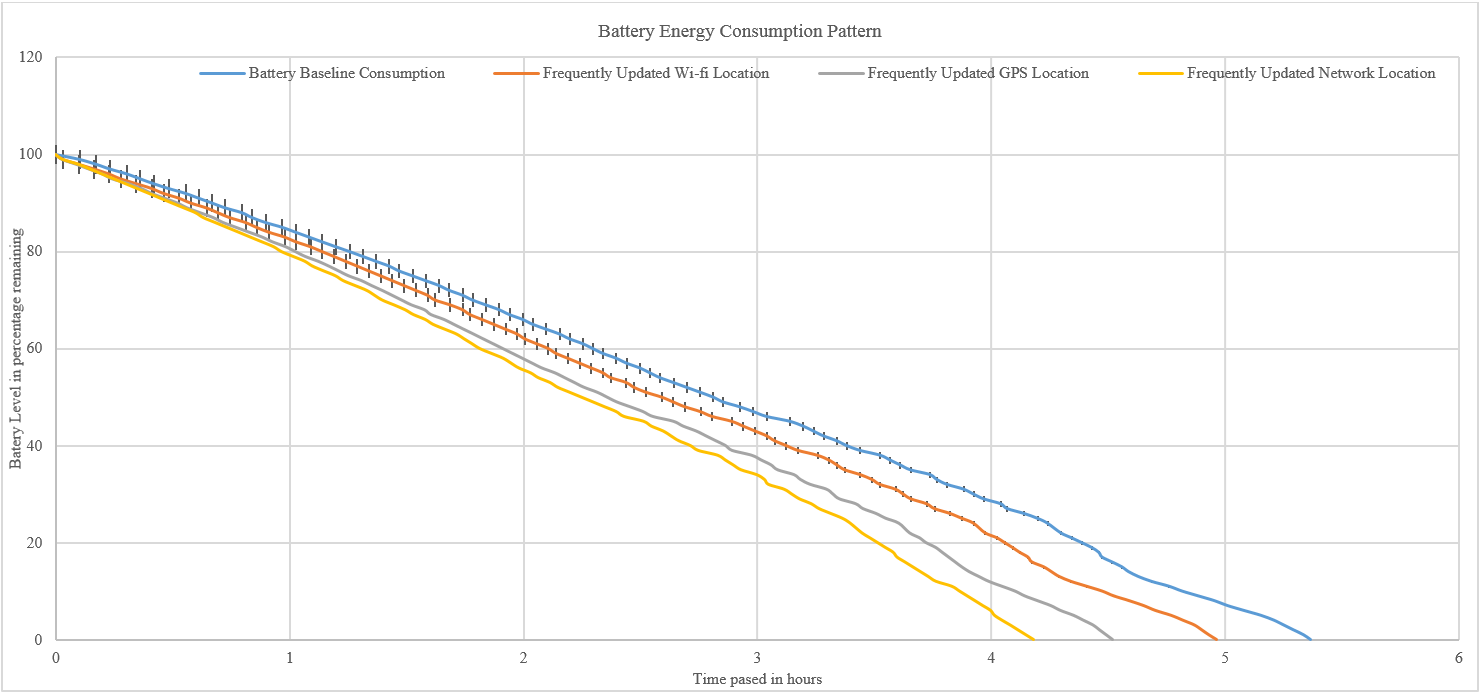
\includegraphics[width=0.9\textwidth]{Battery_Consumption_Pattern.png}
\caption{Change in battery level decrease plotted over time}
\label{fig:battery}
\end{figure*}

From the model we were able to calculate the average values of energy consumption of the sensors under test as follows:-

\begin{table}
\centering
\caption{Average energy consumption data for location sensors in an Android Google Galaxy Nexus phone}
\begin{tabular}{|c|l|} \hline
Sensor&Average (mJ/s)\\ \hline
Baseline Power Consumption&401.12\\ \hline
Wi-Fi Power Consumption&414.15\\ \hline
Network Power Consumption&453.67\\ \hline
GPS Power Consumption&458.67\\ \hline
\hline\end{tabular}
\end{table}

The energy model data was incorporated into our extension of the place ontology explained in the previous section.

\begin{figure*}[tbh]
\centering
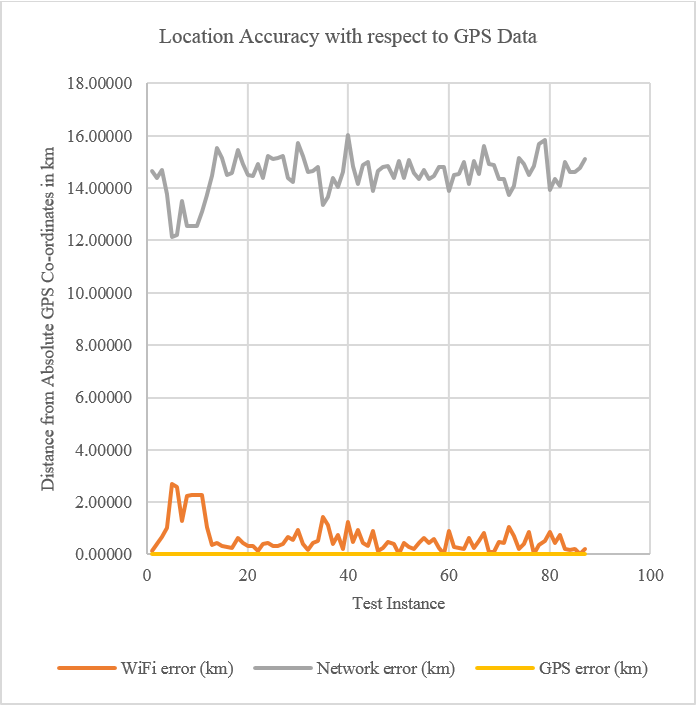
\includegraphics[width=0.9\textwidth]{Accuracy.png}
\caption{Location accuracy for 100 test instances}
\label{fig:accuracy}
\end{figure*}

The other aspect of location sensors that we studied in our work was of location accuracy with respect to a baseline. We observed that although Wi-Fi consumed relatively low energy. It showed fairly accurate location results, given the assumption that we were able to connect to a Wi-Fi location and even if we are connected the Wi-Fi access point has been updated to the Wi-Fi hotspot databases. Network localization on other hand were highly inaccurate and unstable. The high energy cost associated with the network can be attributed to 3G data transmission energy cost. Figure \ref{fig:accuracy} shows the distance predicted, from the absolute location provided by GPS, for Wi-Fi and Network.

\section{Conclusions}

\section{Future Work}

In this project we have provided a design of an energy efficient privacy management solution. We are in process of implementing the middleware for which we have provided the design here. Evaluation of the system poses to be a challenge. We plan to implement two separate systems with and without the context manager middleware and compare and contrast the results to evaluate our system for various privacy manager use cases.

The research work done here is based on the data that can be successfully obtained using Android framework provided data. The best precision of data available through the framework is a one percent change in the battery level. Although the expected battery drain is linear. It may not be exactly linear. We are working on other phones and carrying out research by varying the parameters that affect accuracy and efficiency. We eventually intend to collect enough data to run a learning algorithm and generate a model file. When this model would be put on a phone it will be able to predict the energy consumption patterns of the phones components and adjust the model if necessary.

In course of our research, we observed that frequent update to location context had a significant impact on the battery. GPS position fix although takes substantial time initially \cite{liu2012gps} but once obtained, provides high accuracy in location information. Wi-Fi, on the other hand, had relatively lower precision but got initial position fix faster at known Wi-Fi access point locations. We do take advantage of this trade-off of location precision versus energy measurements to optimize our energy efficiency algorithm. But we have not considered the time to obtain this fix with respect to energy consumption. We would like to study this aspect in the future. We have created the policy-based security mechanism in the Android framework \cite{ghosh2012ms, ghosh2012privacy} and have designed and partially implemented the energy efficient privacy framework. Evaluating this system, however remains to be done.


\bibliographystyle{abbrv}
\bibliography{final_report}

\end{document}